\documentclass{lab_sheet}
\newcommand{\syntax}[1]{
    \lstinputlisting[label={lst:#1},caption={Syntax for #1}, captionpos=b]{./Cmdhelp/#1help.txt}
}
\begin{document}
    \titlePage{Study of Basic Networking Commands}{October 15, 2020}
    \pagenumbering{gobble}
    \tableofcontents
    \pagebreak
    \lstlistoflistings
    \pagebreak
    \listoffigures
    \pagebreak
    \pagenumbering{arabic}
    \section{Objectives}
    \begin{itemize}
        \item Familiarization with basic networking commands and their uses
    \end{itemize}
    \section{Requirements}
    \begin{itemize}
        \item Computer with internet connectivity
    \end{itemize}
    This lab report is prepared based on the networking commands for a Windows OS, more specifically the Windows 10 Home Edition. A list of all the commands used during the lab experiment is presented below:
    \begin{itemize}
        \item ipconfig
        \item ping
        \item getmac
        \item tracert
        \item arp
        \item hostname
        \item netstat
        \item route
    \end{itemize}
    \section{Exercises}
    \problem{Explain the following commands briefly with their functions and few syntaxes.}
    The syntax and options listed in Listing~\ref{lst:ipconfig} to Listing~\ref{lst:route} have been extracted from the command line help with minor changes in the formatting and grammar for ease of understanding.
    \subproblem{ipconfig}
    The \textit{ipconfig} command is used to display the IP address, default gateway and the subnet mask of the different adapters on a device that are bound to TCP/IP. Listing~\ref{lst:ipconfig} shows the syntax along with the options for the \textit{ipconfig} command.
    \syntax{ipconfig}
    \subproblem{ping}
    The \textit{ping} command is used to check the ability of the source system to reach a destination. It works by sending out an ICMP echo request to the destination and waits for a response. Listing~\ref{lst:ping} shows the syntax along with the options for the \textit{ping} command.
    \syntax{ping}
    \subproblem{getmac}
    The \textit{getmac} command is used to display the MAC address, also known as the physical address of the different network adapters on a device. Listing~\ref{lst:getmac} shows the syntax along with the options for the \textit{getmac} command.
    \syntax{getmac}
    \subproblem{tracert}
    The \textit{tracert} command is used to display the details of the path taken by a packet to complete a connection to specified destination. In short, it traces the route of a packet from source to destination. Listing~\ref{lst:tracert} shows the syntax along with the options for the \textit{tracert} command.
    \syntax{tracert}
    \subproblem{arp}
    The \textit{arp} command is used to display and change the ARP(Address Resolution Protocol) cache. ARP uses an IP-to-Physical address translation table to map IP addresses to the corresponding MAC addresses. This command is particularly used to know the MAC addresses of various devices that the system has interacted with based on their IP address and hence is useful in locating duplicate IP addresses. Listing~\ref{lst:arp} shows the syntax along with the options for the \textit{arp} command.
    \syntax{arp}
    \subproblem{hostname}
    The \textit{hostname} command is used to display the host name of the device.  Listing~\ref{lst:hostname} shows the syntax for the \textit{hostname} command. The command doesn't have any additional options for a Windows environment
    \syntax{hostname}
    \subproblem{netstat}
    The \textit{netstat} command is used to display the active TCP network connections, protocol statistics for both IPv4 and IPv6 along with the IP routing table and the listening ports. Listing~\ref{lst:netstat} shows the syntax along with the options for the \textit{netstat} command.
    \syntax{netstat}
    \subproblem{route}
    The \textit{route} command is used to display and manipulate the route informatons on a device. Printing, adding, deleting, or modifying a route is possible using the various command options for \textit{route} command. Listing~\ref{lst:route} shows the syntax along with the options for the \textit{route} command.
    \syntax{route}
    \problem{Note down the observation of each steps performed during the experiment along with necessary commands and also comment on it.}
    \subproblem{Using ipconfig}
    \cmdop{ipa}{ipconfig}
    Listing~\ref{lst:ipa} shows the observation for \textit{ipconfig}. The IP addresses, subnet mask, and default gateways are displayed when the command is executed. There are multiple network adapters on the system, all of which are seen in the listing. The wireless LAN adapter is the one of concern in this observation since the system is connected to the internet via the Wi-Fi adapter. The IPv4 address of the adapter is 192.168.1.19 with the default gateway 192.168.1.1, which will be useful in further observations.
    \cmdop{ipb}{ipconfig/all}
    Listing~\ref{lst:ipb} shows the observation for \textit{ipconfig/all}. The \textit{/all} option for the \textit{ipconfig} command displays additional informations about the various network adapters on the system. For instance, the descriptive name, physical address, DHCP status, autoconfiguration status, DNS servers and more for each adapter are displayed in addition to the original observation in Listing~\ref{lst:ipa}.
    \subproblem{Using ping}
    \cmdop{pinga}{ping to default gateway}
    As discussed earlier, the \textit{ping} command tests the ability of a source to reach a destination. In Listing~\ref{lst:pinga} the system is pinging the default gateway, i.e. 192.168.1.1 which was previously observed in Listing~\ref{lst:ipa}. The statistics such as number of packets sent and received before timeout, approximate round trip time in milli-seconds for the packet to reach from the source address to the default gateway address is displayed. It is obvious that this link will have less RTT, which can also be observed in the Listing~\ref{lst:pinga}.
    \cmdop{pingb}{ping to vianet.com.np}
    The ISP subscribed while performing this experiment is Vianet Communications Pvt. Ltd. So, pinging their website vianet.com.np gives the observation shown in Listing~\ref{lst:pingb}. This link generally takes less RTT since the system has a faster link to the subscribed ISP, which can be verified from the observation.
    \cmdop{pingc}{ping to google.com}
    Listing~\ref{lst:pingc} shows the observation for pinging google.com website. The number of packets sent, received and lost along with the estimated RTT is shown in the observation, and clearly the RTT is higher than that with the default gateway and ISP. 
    \cmdop{pingd}{ping to 103.5.150.3}
    Listing~\ref{lst:pingd} shows the observation for pinging an IP 103.5.150.3, which is one of the multiple IP addressess owned by Pulchowk Campus. A notable observation here can be made in comparision to Listing~\ref{lst:pingb} and Listing~\ref{lst:pingc}, where domain names were used to ping the server. But in fact, the server's IP address was being resolved which was truly being pinged. So, a ping to either the actual server IP or a domain name is possible and it is due to the DNS resolution technique used by the process. 
    \subproblem{Using getmac}
    \cmdop{gmac}{getmac}
    Listing~\ref{lst:gmac} shows the observation for \textit{getmac} command. The physical addressess for the various network adapters are displayed. The same addresses are also observed in the Listing~\ref{lst:ipb} under individual adapter section.
    \subproblem{Using tracert}
    \cmdop{tracerta}{tracert to default gateway}
    Listing~\ref{lst:tracerta} shows the observation for \textit{tracert} to the default gateway. It is obvious that this should complete in one hop since a gateway is essentially one hop away from the IP address of the system. This is verified from the observation as well.
    \cmdop{tracertb}{tracert to vianet.com.np}
    Listing~\ref{lst:tracertb} shows the observation for \textit{tracert} to the ISPs website, i.e. vianet.com.np. The number of hops taken by a packet leaving a system to reach it's subscribed ISPs website is generally lower than any other websites. This is seen from the observation as well, since the packet only takes 4 hops to reach the destination.
    \cmdop{tracertc}{tracert to google.com}
    Listing~\ref{lst:tracertc} shows the observation for \textit{tracert} to google.com. The packet takes 17 hops to reach the destination and as observed, takes a route that passes through the subscribed ISP's subnet before hoping on to another IP to reach the destination. 
    \cmdop{tracertd}{tracert to 103.5.150.3}
    Listing~\ref{lst:tracertd} shows the observation for \textit{tracert} to 103.5.150.3. It is seen that the packet hops on a Nepal Telecommunications Corporation IP which shows that the ISP for the destination IP is Nepal Telecommunications.
    A notable informations that can be gathered from the \textit{tracert} command executions shown in Listing~\ref{lst:tracerta} to Listing~\ref{lst:tracertd} is that the packet initially hops on the default gateway address 192.168.1.1 regardless of the destination. This is true since the gateway is essentially a bridge for the private network and the internet.
    \subproblem{Using arp}
    \cmdop{arpa}{arp -a}
    Listing~\ref{lst:arpa} shows the observation for \textit{arp -a} command. The IP-to-Physical address table for all devices or modules that the various network adapter interfaces have interacted and thus stored in the ARP table are displayed. The wireless LAN adapter which is the second entry, is seen to interact with the default gateway. The physical address c8-50-e9-63-da-9a is indeed the MAC address of the router used for the wirless connection. 
    \cmdop{arpb}{ping to another device on the network followed by arp -a}
    Listing~\ref{lst:arpb} shows the observation for \textit{arp -a} command after another device on the same network was pinged. The IP address obtained by a mobile device on the network was 192.168.1.13, which is pinged from the system. After that, execution of the \textit{arp -a} command shows that the wireless LAN adapter has an additional entry in its ARP table which gives the IP and the physical address of the mobile device that was pinged.
    \subproblem{Using hostname}
    \cmdop{hname}{hostname}
    Listing~\ref{lst:hname} shows the observation for \textit{hostname} command. The hostname for the system on which the experiment was performed is LAPTOP-QLRVLCUC.
    \subproblem{Using netstat}
    \cmdop{netstata}{netstat -a}
    Listing~\ref{lst:netstata} shows the observation for \textit{netstat -a} command. All the active ports with the local address, foreign address and the status along with the protocol used are displayed. The same IP has been used with varying port numbers to establish different connections on the system which is clear from the observation.
    \cmdop{netstatb}{netstat -e}
    Listing~\ref{lst:netstatb} shows the observation for \textit{netstat -e} command. The network connection statistics such as bytes of data sent and received, unicast packets, non-unicast packets and any discards or error are observed by executing the \textit{netstat -e} command.
    \cmdop{netstatc}{netstat -r}
    Listing~\ref{lst:netstatc} shows the observation for \textit{netstat -r} command. The routing table information such as interfaces available, active routes, persistent routes, including both the IPv4 and IPv6 route tables are displayed.
    \subproblem{Using route}
    \cmdop{routea}{route print}
    Listing~\ref{lst:routea} shows the observation for \textit{route print} command. The execution results in an observation similar to the \textit{netstat -r} command, which also prints the route table informations. The command defaults to display both the IPv4 and IPv6 routing tables.
    \cmdop{routeb}{route print -4}
    Listing~\ref{lst:routeb} shows the observation for \textit{route print -4} command. The additional parameter on this command displays only the IPv4 route table.
    \cmdop{routec}{route print -6}
    Listing~\ref{lst:routec} shows the observation for \textit{route print -6} command. The additional parameter on this command displays only the IPv6 route table.
    \problem{What is the actual IP address of your computer? Also find the Public IP address that is being used for your computer’s Internet connectivity. Note down both the IP addresses.}
    The actual IP address of the system on which the experiments were performed is observed in Listing~\ref{lst:ipa} and Listing~\ref{lst:ipb}.
    There are a few different methods to check the public IP address. 
    \subproblem{Using the Command Prompt (nslookup) and OpenDNS service}
    The command \textit{nslookup myip.opendns.com resolver1.opendns.com} can be used to know the public IP of a system.
    \cmdop{publicipa}{public IP address using nslookup and OpenDNS service}
    \subproblem{Using the Powershell}
    On a Windows platform, the Powershell command \textit{(Invoke-WebRequest ifconfig.me/ip).Content.Trim()} gives the public IP address of the system.
    \cmdop{publicipb}{public IP address using Powershell}
   \subproblem{Using third party websites}
    There are numerous websites that can be used to check the public IP address that the system is using to interact on the internet. Google has a service that allows users to check their public IP address by simply searching for \textit{my ip} or \textit{what is my ip} using the google search engine.
    \begin{figure}[H]
        \centering
        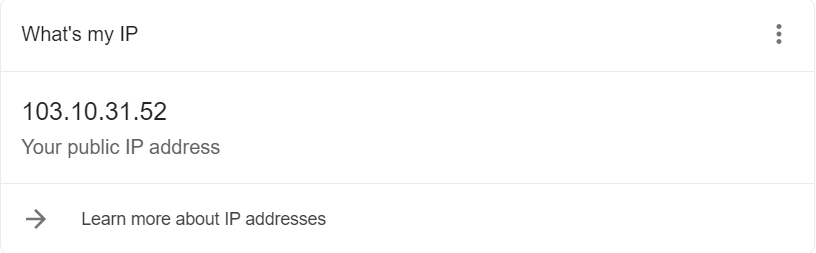
\includegraphics[scale=0.8,frame]{./Figures/publicip.png}
        \label{fig:publicip}
        \caption{Observation for public IP address using google search engine}
    \end{figure}
    From this, the following remarks can be made,\\
    \textbf{Actual IP address:} 192.168.1.19\\
    \textbf{Public IP address:} 103.10.31.52
    \section{Conclusion}
    The various networking commands that can be used to know the IP addresses, MAC addresses, configuration status of adapters, check for internet connectivity, trace the route of packets that are sent over the network to a specified destination, display and manipulate the Address Resolution Protocol cache table, route tables were discussed and executed throughout the lab. This report encompasses all the observations made during the experiment with some key comments on the functioning and behavior of the aforementioned commands.
\end{document}